\documentclass[../report.tex]{subfiles}
\begin{document}
    
    \begin{frame}
        \frametitle{5a: Frame Interpolation}
        \begin{figure}[!htb]
            \centering
            \frame{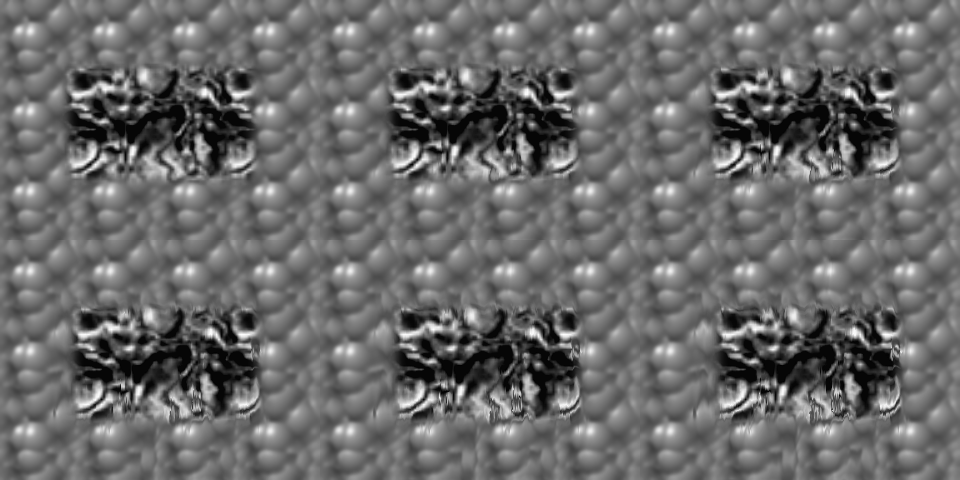
\includegraphics[keepaspectratio,height=0.65\textheight,width=0.80\textwidth]{ps4-5-a-1}}
            \caption{ps4-5-a-1}
        \end{figure}
    \end{frame}

    \begin{frame}
        \frametitle{5b: Frame Interpolation}
        \begin{figure}[!htb]
            \centering
            \frame{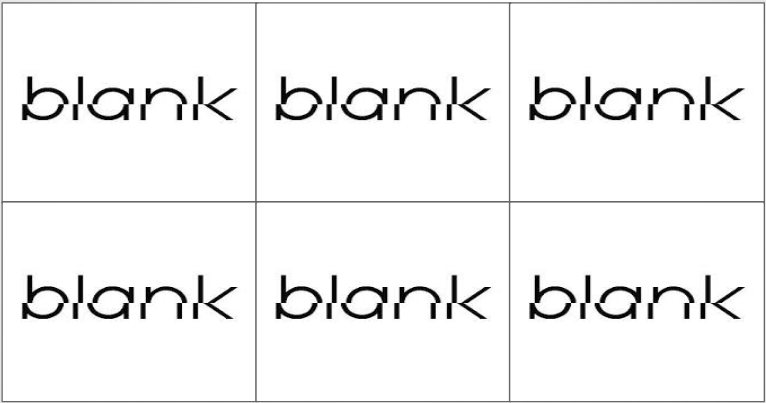
\includegraphics[keepaspectratio,height=0.65\textheight,width=0.80\textwidth]{ps4-5-b-1}}
            \caption{ps4-5-b-1}
        \end{figure}
    \end{frame}

    \begin{frame}
        \frametitle{5b: Frame Interpolation}
        \begin{figure}[!htb]
            \centering
            \frame{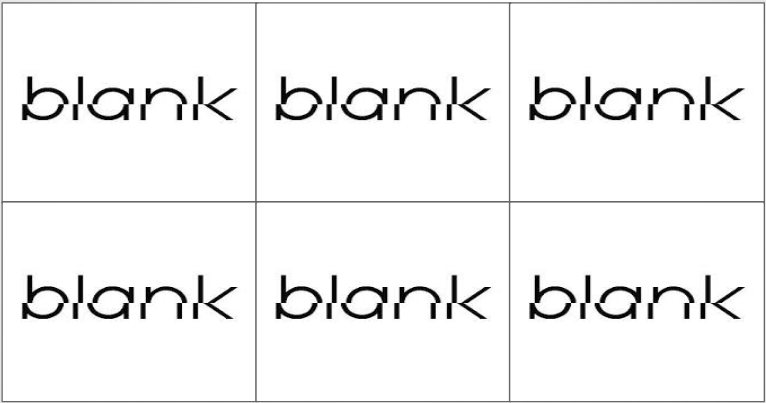
\includegraphics[keepaspectratio,height=0.65\textheight,width=0.80\textwidth]{ps4-5-b-2}}
            \caption{ps4-5-b-2}
        \end{figure}
    \end{frame}

\end{document}